% Progress presentation, 04/11 -> 12/11/2026. Reuses the paper's figures and tables:
% rerun scripts/make_paper_tables.py and compile the figures in paper/figures first.
%   cd presentation && latexmk -pdf avancos_2026-11-12.tex
\documentclass[aspectratio=169,10pt]{beamer}
\usepackage[T1]{fontenc}
\usepackage[utf8]{inputenc}
\usepackage[brazil]{babel}
\usepackage{booktabs,multirow,array,graphicx,amsmath,bm}
\usepackage{xcolor}
% Shared macros. Change \model once to rename the architecture everywhere.
\newcommand{\model}{COVER}
\newcommand{\todo}[1]{\textcolor{red}{[TODO: #1]}}

% Labels and sets
\newcommand{\E}{\textsc{e}}
\newcommand{\N}{\textsc{n}}
\newcommand{\C}{\textsc{c}}
\newcommand{\Prem}{\mathcal{P}}
\newcommand{\Hyp}{\mathcal{H}}
\newcommand{\Rel}{\mathcal{R}}
\newcommand{\Ops}{\mathcal{O}}
\newcommand{\cls}{\textsc{[cls]}}
\newcommand{\nullnode}{\varnothing}
\newcommand{\Lset}{\mathcal{L}_{\mathrm{set}}}
\newcommand{\Pcov}{P_{\mathrm{cov}}}
\newcommand{\Pnc}{P_{\neg\mathrm{conf}}}
\newcommand{\LN}{\operatorname{LN}}
\newcommand{\MLP}{\operatorname{MLP}}
\newcommand{\softplus}{\operatorname{softplus}}
\newcommand{\vect}[1]{\bm{#1}}

\renewcommand{\todo}[1]{}
\renewcommand{\cls}{[CLS]}

\definecolor{neural}{HTML}{2F6DB5}
\definecolor{symb}{HTML}{D9822B}
\definecolor{logic}{HTML}{2E8B57}
\definecolor{relneg}{HTML}{C0392B}

\usetheme{default}
\setbeamercolor{background canvas}{bg=white}
\setbeamercolor{frametitle}{fg=black}
\setbeamercolor{title}{fg=black}
\setbeamercolor{structure}{fg=neural}
\setbeamerfont{frametitle}{series=\bfseries,size=\large}
\setbeamertemplate{navigation symbols}{}
\setbeamertemplate{itemize items}[circle]
\setbeamertemplate{footline}{\hfill\textcolor{black!45}{\scriptsize\insertframenumber/\inserttotalframenumber}\hspace{1em}\vspace{0.6em}}

\newcommand{\up}[1]{\textcolor{logic}{\textbf{#1}}}
\newcommand{\down}[1]{\textcolor{relneg}{\textbf{#1}}}
\newcommand{\take}[1]{\vspace{4pt}\begin{beamercolorbox}[sep=5pt,rounded=true]{take}\small #1\end{beamercolorbox}}
\setbeamercolor{take}{bg=black!5,fg=black}
% paper tables are tabular* at \textwidth: typeset them wide, then scale to the slide
\newcommand{\tbl}[3][1]{{\setlength{\textwidth}{#2}\resizebox{#1\linewidth}{!}{\input{../paper/tables/#3}}}}

\title{Experimentos em Natural Language Inference (NLI)}
\author{}
\date{17 de novembro de 2026}

\begin{document}

\begin{frame}[plain]
  \centering\vfill
  {\fontsize{30}{36}\selectfont\bfseries Experimentos em\\[4pt] Natural Language Inference (NLI)\par}
  \vspace{1.2cm}
  {\large 17 de novembro de 2026\par}
  \vfill
\end{frame}

% --------------------------------------------------------------------------


% --------------------------------------------------------------------------
\begin{frame}{\model{}: a ideia}
\centering
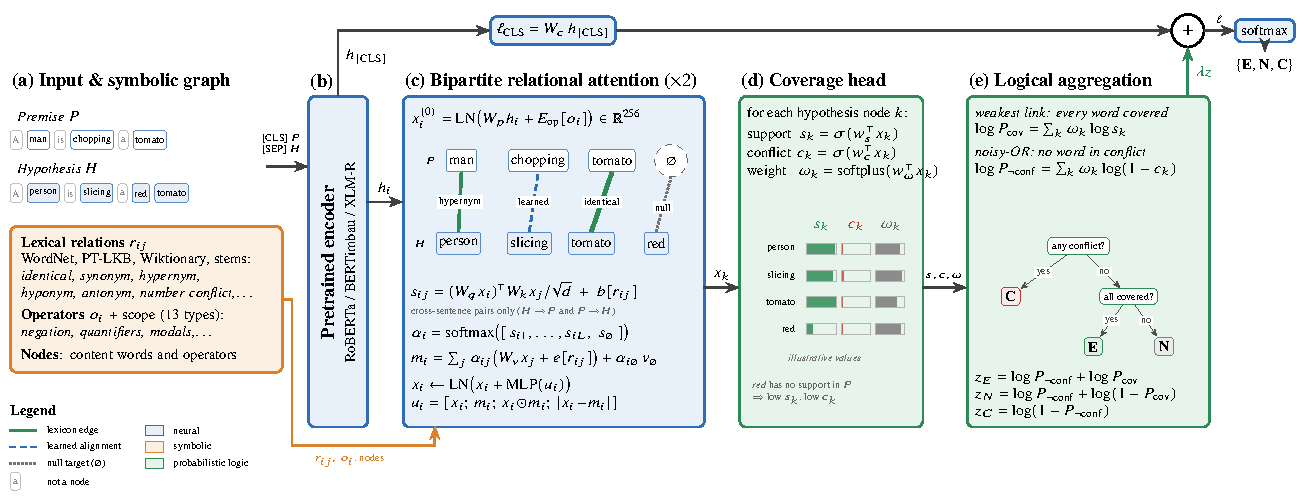
\includegraphics[width=\linewidth]{../paper/figures/cover_architecture.pdf}
\vspace{2pt}
\small
Para cada palavra da hipótese: \textcolor{logic}{\textbf{suporte}} (a premissa cobre?) e
\textcolor{relneg}{\textbf{conflito}} (a premissa contradiz?) $\Rightarrow$ regra lógica:
\E{} = tudo coberto e sem conflito; \N{} = algo não coberto; \C{} = algum conflito.
\end{frame}

% --------------------------------------------------------------------------


% --------------------------------------------------------------------------


% --------------------------------------------------------------------------


% --------------------------------------------------------------------------


% --------------------------------------------------------------------------
\begin{frame}{Desenho das experimentações}
\centering
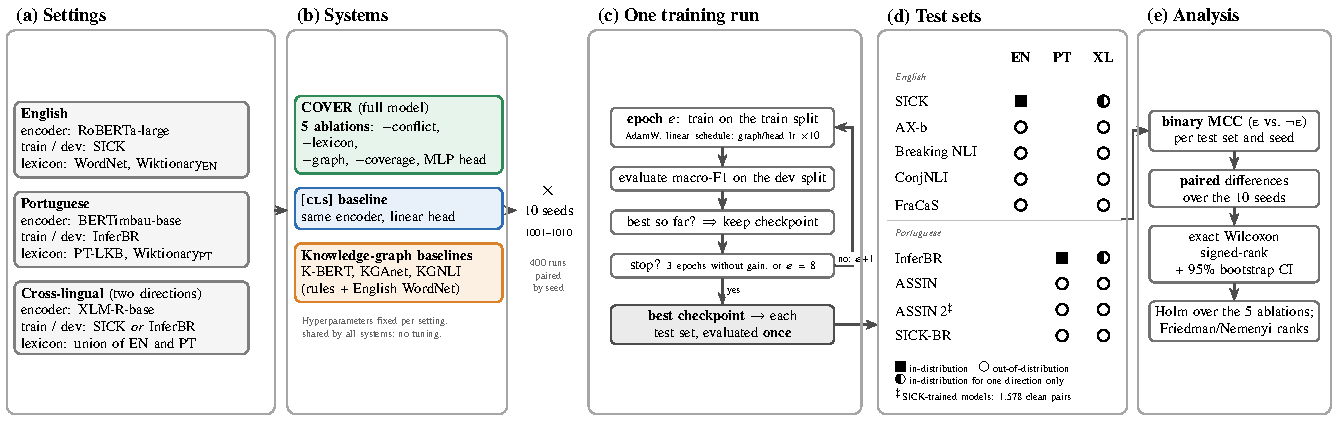
\includegraphics[width=\linewidth]{../paper/figures/experimental_design.pdf}
\small
Hiperparâmetros fixos por configuração, sem ajuste por variante; tudo pareado por seed.
\end{frame}

% --------------------------------------------------------------------------
\begin{frame}{Conjuntos de teste}
\begin{columns}[T]
\column{0.5\textwidth}
\small
\begin{tabular}{@{}llrl@{}}
\toprule
Conjunto & Língua & Pares & Testa \\
\midrule
SICK & EN & 4.906 & in-distribution \\
AX-b & EN & 1.104 & fenômenos linguísticos \\
\textbf{Breaking NLI} & EN & 8.193 & troca de 1 palavra \\
\textbf{ConjNLI} & EN & 623 & conjunções \\
\textbf{FraCaS} & EN & 335 & semântica formal \\
\midrule
InferBR & PT & 1.705 & in-distribution \\
ASSIN & PT & 4.000 & OOD \\
ASSIN\,2 & PT & 2.448 & OOD \\
\textbf{SICK-BR} & PT & 4.906 & tradução do SICK \\
\bottomrule
\end{tabular}
\column{0.46\textwidth}
\small
\begin{itemize}
\item Em negrito: conjuntos de desafio adicionados.
\item HANS e MED foram testados e retirados (tempo de avaliação).
\item SICK-BR é alinhado par a par com o SICK.
\item \textbf{Métricas}: acurácia e MCC da decisão binária \E{} vs.\ $\neg$\E{}, as únicas definidas em todos os conjuntos.
\end{itemize}
\end{columns}
\end{frame}

% --------------------------------------------------------------------------
\begin{frame}{Resultados principais --- inglês}
\textit{\small (a) English: RoBERTa-large trained on SICK} \hfill {\scriptsize $^\dagger$ $p<.05$ contra [CLS]}\\[3pt]
\tbl{18.5cm}{main_en}
\take{SICK: \textbf{empate}. Fora da distribuição: \up{+4.9} AX-b, \up{+5.9} ConjNLI, \up{+8.6} FraCaS (MCC). Breaking NLI: empate. \textbf{Baselines de grafo}: empatam (ou quase) no SICK mas caem fora dele; \model{} supera KGAnet, KGNLI e K-BERT em \up{+10} a \up{+21} MCC em AX-b e ConjNLI (10/10 seeds).}
\end{frame}

% --------------------------------------------------------------------------
\begin{frame}{Resultados principais --- português}
\textit{\small (b) Portuguese: BERTimbau-base trained on InferBR} \hfill {\scriptsize $^\dagger$ $p<.05$ contra [CLS]}\\[3pt]
\tbl{16.5cm}{main_pt}
\take{InferBR: \textbf{empate} (+1.2 MCC, n.s.). Fora da distribuição: \up{+3.3} ASSIN, \up{+4.6} ASSIN\,2, \up{+5.3} SICK-BR (MCC), com $\sim$1/3 do desvio entre seeds.}
\end{frame}

% --------------------------------------------------------------------------
\begin{frame}{Transferência entre línguas}
\scriptsize
\textit{(c) Cross-lingual EN$\to$PT: XLM-R-base trained on SICK, Portuguese tests}\\[1pt]
\tbl{16.5cm}{main_xl_en_to_pt}\\[5pt]
\textit{(d) Cross-lingual PT$\to$EN: XLM-R-base trained on InferBR, English tests}\\[1pt]
\tbl{18.5cm}{main_xl_pt_to_en}
\take{EN$\to$PT: \textbf{empate} com o [CLS] nos testes em português (ASSIN\,2 só nos pares que não vêm do treino do SICK); K-BERT e KGAnet ficam $\sim$20--27 MCC abaixo no InferBR e no SICK-BR (KGNLI em execução). PT$\to$EN (10 seeds): \model{} ganha no SICK \up{+4.7} e no ConjNLI \up{+6.3}; AX-b e FraCaS positivos mas n.s.; Breaking NLI empate. Confirma a direção promissora dos testes preliminares.}
\end{frame}

% --------------------------------------------------------------------------
\begin{frame}{Ablação: o que cada variante remove}
\centering
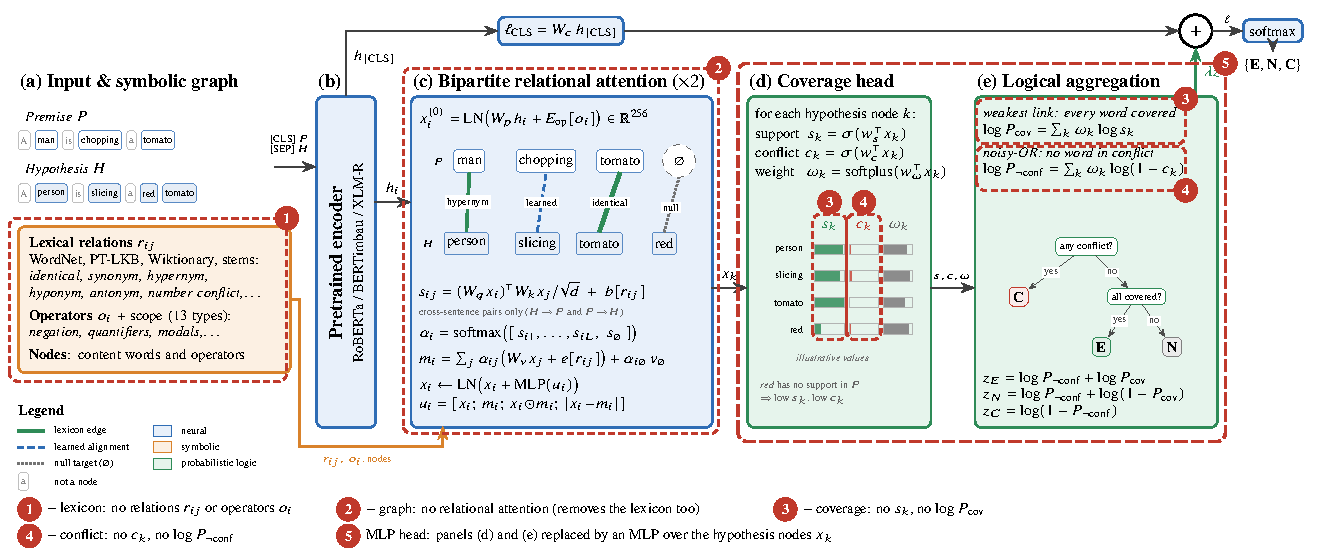
\includegraphics[width=\linewidth]{../paper/figures/ablation_architecture.pdf}
\end{frame}

% --------------------------------------------------------------------------
\begin{frame}{Ablação ($\Delta$ MCC contra o \model{} completo)}
\scriptsize
\textit{(a) English: RoBERTa-large trained on SICK}\\[1pt]
\tbl[0.9]{12cm}{ablation_en}\\[4pt]
\textit{(b) Portuguese: BERTimbau-base trained on InferBR}\\[1pt]
\tbl[0.9]{12cm}{ablation_pt}\\[2pt]
{\tiny $^*$Holm $p<.05$ contra o completo; $^\dagger$ $p<.05$.}
\end{frame}

% --------------------------------------------------------------------------
\begin{frame}{Ablação na transferência EN$\to$PT (XLM-R treinado em SICK)}
\textit{\small Testes em português; $\Delta$ MCC contra o \model{} completo} \hfill {\scriptsize $^*$Holm $p<.05$; $^\dagger$ $p<.05$ contra o completo}\\[3pt]
\tbl[0.85]{12cm}{pres_ablation_xl_en_to_pt}
\take{Ablação completa. Na transferência para o português \textbf{nenhum componente ajuda}: nenhuma variante é significativamente pior que o \model{} completo, e tirar o grafo ou o léxico até melhora o SICK-BR (\up{+2.1}, Holm). As relações aprendidas em inglês não parecem transferir para as arestas em português.}
\end{frame}

% --------------------------------------------------------------------------
\begin{frame}{Ablação na transferência PT$\to$EN (XLM-R treinado em InferBR)}
\textit{\small Testes em inglês; $\Delta$ MCC contra o \model{} completo} \hfill {\scriptsize $^*$Holm $p<.05$; $^\dagger$ $p<.05$ contra o completo}\\[3pt]
\tbl[0.85]{12cm}{pres_ablation_xl_pt_to_en}
\take{Parcial (2 de 5 ablações completas). Aqui o \textbf{léxico é essencial}: sem ele o modelo perde SICK \down{$-$4.5} e ConjNLI \down{$-$6.8} (Holm, 10/10 seeds), quase todo o ganho do \model{} sobre o [CLS]. Sem o conflito: melhor em 4 de 5 testes (n.s.), pior no FraCaS. Restante em execução.}
\end{frame}

% --------------------------------------------------------------------------
\begin{frame}{Ablação: o que aprendemos}
\small
\footnotesize\setlength{\tabcolsep}{3pt}\begin{tabular}{@{}>{\raggedright\arraybackslash}p{1.6cm}>{\raggedright\arraybackslash}p{3.3cm}>{\raggedright\arraybackslash}p{3.3cm}>{\raggedright\arraybackslash}p{2.5cm}>{\raggedright\arraybackslash}p{2.7cm}@{}}
\toprule
Componente & Inglês (RoBERTa-large) & Português (BERTimbau) & EN$\to$PT (XLM-R) & PT$\to$EN (XLM-R) \\
\midrule
\textbf{Cobertura} & \down{essencial}: sem ela AX-b $-$6.7, Conj.\ $-$8.5, FraCaS $-$9.6 & \down{essencial}: ASSIN $-$11.9, ASSIN\,2 $-$4.0, SICK-BR $-$4.2 & n.s. & \textit{em execução} \\
\textbf{Regra lógica} & \down{essencial}: MLP head AX-b $-$5.1, Conj.\ $-$11.8 & secundária: MLP head $-$0.8 a $-$2.4 (n.s.) & n.s. & \textit{em execução} \\
\textbf{Grafo} & ajuda no ConjNLI ($-$4.8) & ajuda fora da distribuição ($-$1.8 a $-$2.1) & \down{atrapalha} (sem ele: SICK-BR +2.1) & \textit{em execução} \\
\textbf{Léxico} & não faz diferença & ajuda ($-$1.3 a $-$1.5) & \down{atrapalha} (sem ele: SICK-BR +2.1) & \down{essencial}: SICK $-$4.5, Conj.\ $-$6.8 \\
\textbf{Conflito} & \up{dispensável} (sem ele: +2.0 AX-b) & \up{dispensável} (sem ele: +1.0 a +2.4) & n.s. & n.s. (sem ele: $+$1.6 a $+$6.0; FraCaS $-$3.1) \\
\bottomrule
\end{tabular}
\take{O ganho vem da \textbf{cobertura}; o conflito não ajuda em nenhuma configuração (nos testes preliminares em português parecia ajudar). Na transferência EN$\to$PT nenhum componente ajuda; na PT$\to$EN o léxico (EN+PT) é o que carrega a transferência. Pergunta em aberto: retirar o conflito do modelo principal?}
\end{frame}

% --------------------------------------------------------------------------
\begin{frame}{Análise de erros: AX-b por fenômeno (inglês, MCC)}
\begin{columns}[T]
\column{0.48\textwidth}
\small
\begin{tabular}{@{}lrccc@{}}
\toprule
Categoria & $n$ & [CLS] & \model{} & $\Delta$ \\
\midrule
Lexical semantics & 368 & 47.7 & 50.2 & \up{+2.5} \\
Predicate--argument & 424 & 45.4 & 51.7 & \up{+6.3} \\
Logic & 364 & 19.9 & 26.2 & \up{+6.3} \\
Knowledge & 284 & 29.5 & 31.5 & +2.0 \\
\bottomrule
\end{tabular}
\column{0.48\textwidth}
\small
\begin{tabular}{@{}lrr@{}}
\toprule
Fenômeno & $n$ & $\Delta$ \\
\midrule
Genitives/Partitives & 20 & \up{+33.1} \\
Nominalization & 28 & \up{+28.2} \\
Morphological negation & 26 & \up{+24.3} \\
Temporal & 32 & \up{+24.1} \\
Double negation & 28 & \up{+22.5} \\
\midrule
Restrictivity & 26 & \down{$-$15.8} \\
Universal & 18 & \down{$-$10.1} \\
Symmetry/Collectivity & 28 & \down{$-$8.7} \\
\bottomrule
\end{tabular}
\end{columns}
\take{Ganho concentrado em estrutura e lógica, não em conhecimento lexical. Fenômenos com $n<40$ são exploratórios (tabela completa no artigo).}
\end{frame}

% --------------------------------------------------------------------------


% --------------------------------------------------------------------------
\begin{frame}{Interpretabilidade}
\begin{columns}[c]
\column{0.55\textwidth}
\centering
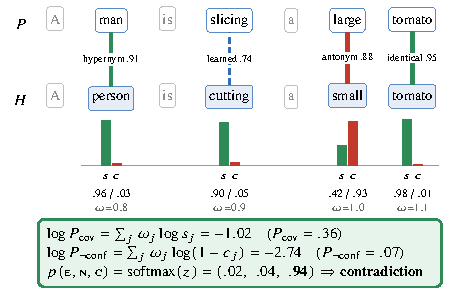
\includegraphics[width=\linewidth]{../paper/figures/interpretability_example.pdf}\\
{\tiny valores ilustrativos}
\column{0.43\textwidth}
\small
\begin{itemize}
\item Cada decisão se lê palavra por palavra: quem cobre, quem contradiz.
\item A parte estruturada é quem decide de fato: sozinha, MCC \textbf{.84} no SICK contra \textbf{.45} da parte \cls{}.
\item Ela muda 29\% das decisões do \cls{}: corrige 25\%, estraga 3\%.
\end{itemize}
\end{columns}
\end{frame}

% --------------------------------------------------------------------------
\begin{frame}{Conclusões até agora}
\small
\begin{enumerate}
\item \textbf{Padrão robusto:} \model{} empata no conjunto de treino e ganha fora dele, em inglês e em português, com três encoders.
\item \textbf{O mecanismo é a cobertura}; a regra lógica pesa no inglês; grafo e léxico ajudam no português.
\item \textbf{O conflito não ajuda} (diferente dos testes preliminares em português).
\item \model{} tem \textbf{menor variância entre seeds} (ex.: SICK-BR $\pm$0.8 vs.\ $\pm$3.2).
\item \textbf{Cross-lingual:} EN$\to$PT não transfere; PT$\to$EN transfere (SICK \up{+4.7}, ConjNLI \up{+6.3}).
\item \textbf{Baselines de grafo} (KGAnet, KGNLI): empatam no SICK, mas ficam abaixo até do [CLS] fora da distribuição.
\item Correção metodológica: 36\% do teste do ASSIN\,2 vem do treino do SICK; modelos treinados em SICK são avaliados só no restante.
\end{enumerate}
\end{frame}

% --------------------------------------------------------------------------
\begin{frame}{Início da escrita do artigo}
\begin{columns}[c]
\column{0.62\textwidth}
\centering
\fbox{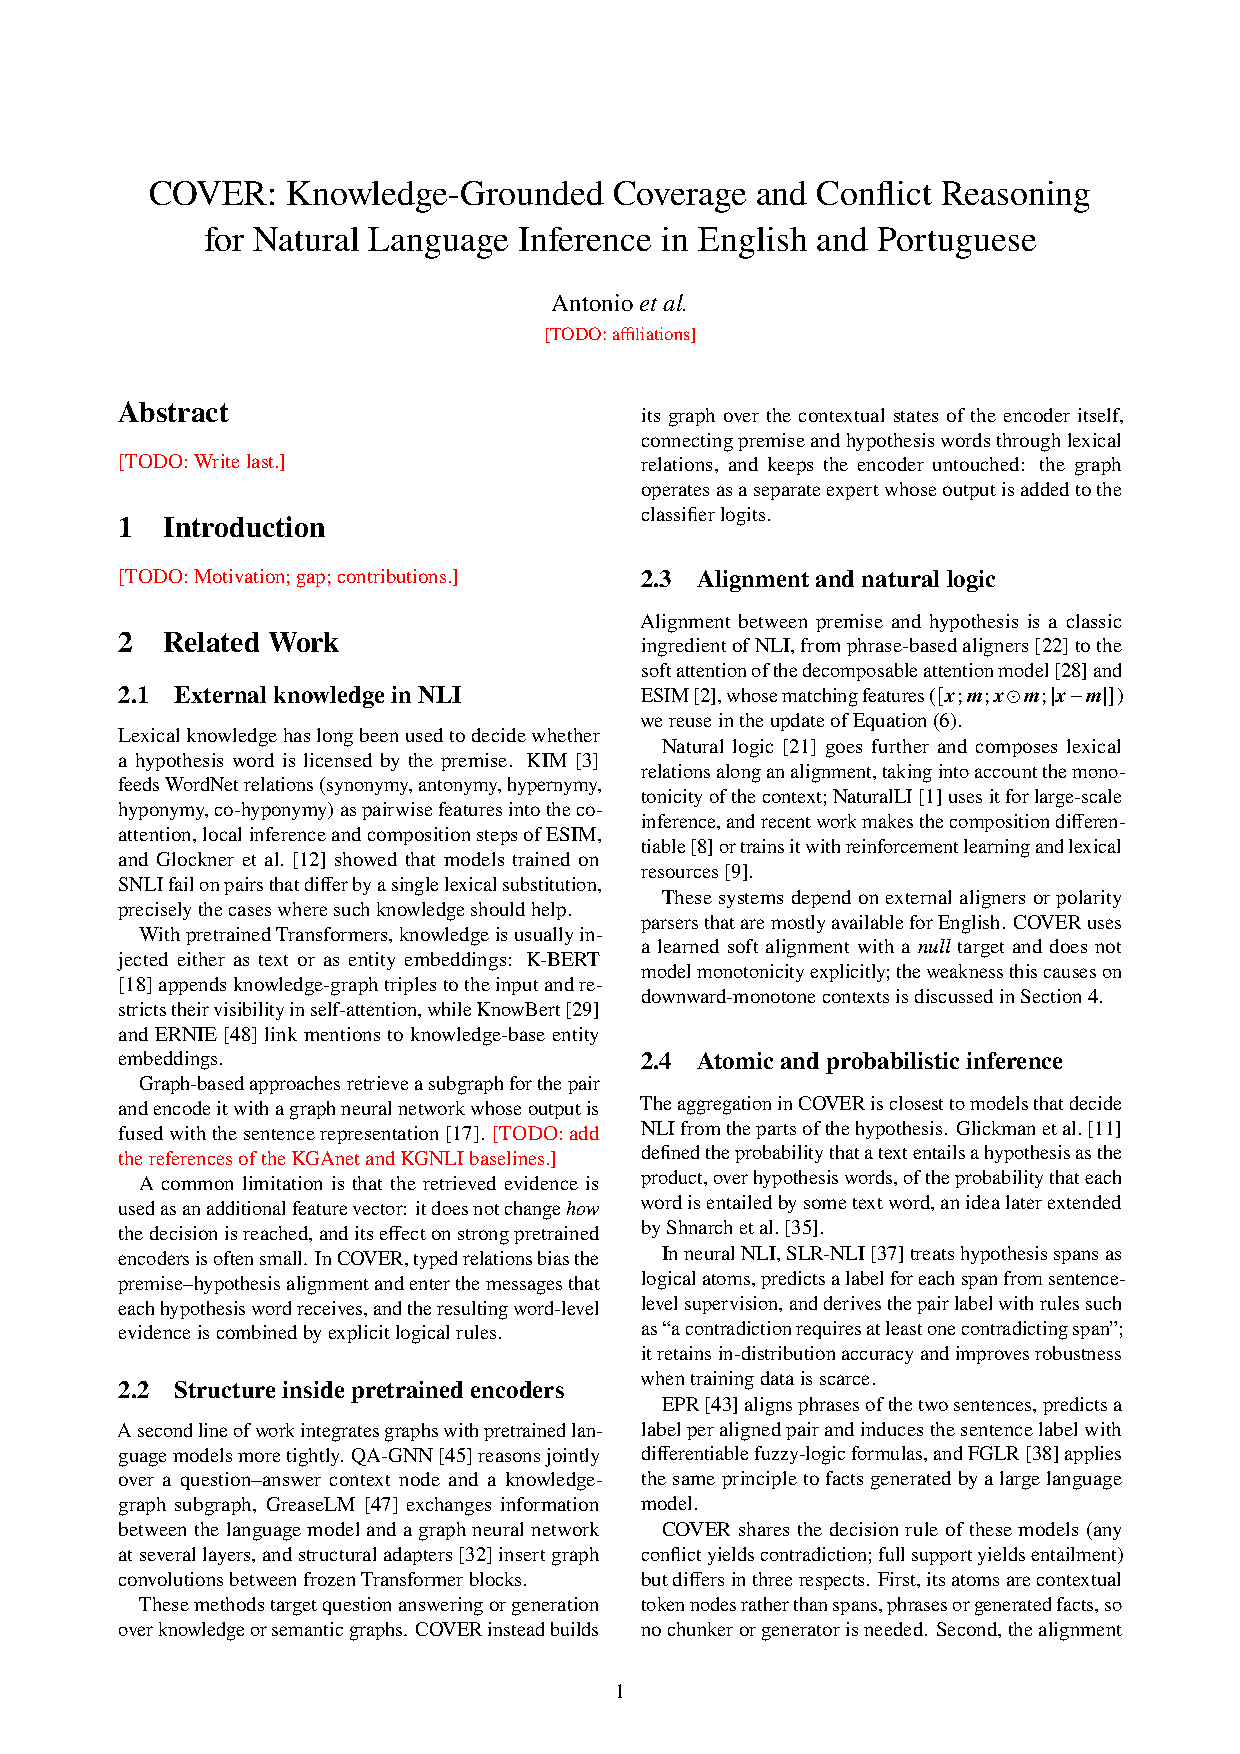
\includegraphics[width=0.46\linewidth]{img/artigo_p1.png}}\hfill%
\fbox{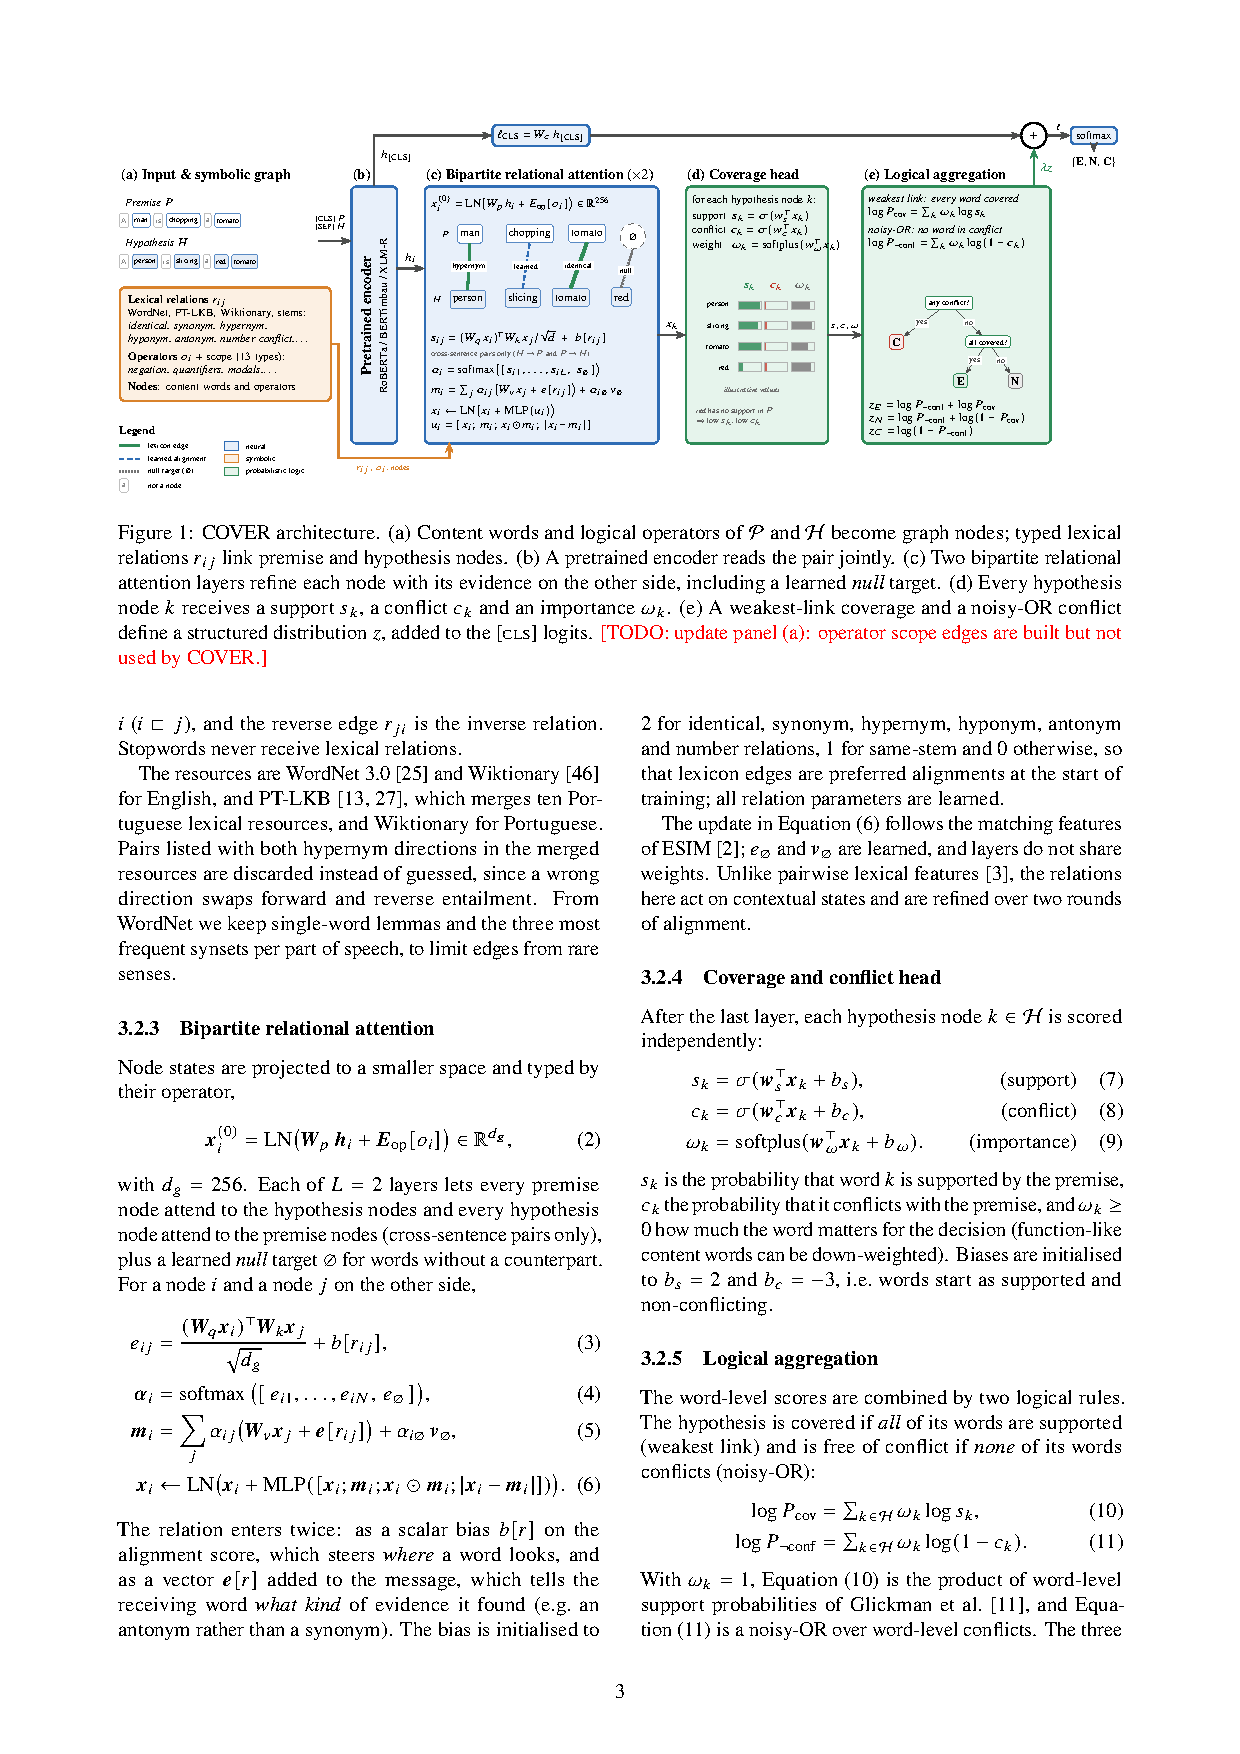
\includegraphics[width=0.46\linewidth]{img/artigo_p3.png}}
\column{0.36\textwidth}
\footnotesize
\textit{\model{}: Knowledge-Grounded Coverage and Conflict Reasoning for NLI in English and Portuguese}\\[6pt]
\textbf{Já escrito}
\begin{itemize}
\item Trabalhos relacionados
\item Metodologia: arquitetura, treino, ablações, baselines, protocolo
\item 4 figuras e as tabelas de resultados, geradas automaticamente dos experimentos
\end{itemize}
\textbf{A fazer}
\begin{itemize}
\item Texto dos resultados e discussão
\item Introdução, resumo e conclusão
\end{itemize}
\end{columns}
\end{frame}

% --------------------------------------------------------------------------
\begin{frame}{Próximos passos}
\small
\begin{itemize}
\item Concluir as experimentações (duas máquinas, previsão 14--15/11): ablação PT$\to$EN e baselines de grafo no português e no cross-lingual; K-BERT no inglês.
\item Decidir o papel do conflito: manter, tornar opcional ou retirar do modelo principal.
\item Corrigir o viés de numerais (\texttt{number\_conflict}) numa versão 2.
\item Artigo: escrever o texto dos resultados; exportar valores reais para a figura de interpretabilidade; calibração (ECE melhor fora da distribuição).
\item Pendências do artigo: referências de KGAnet/KGNLI e do InferBR.
\end{itemize}
\end{frame}

\end{document}
